\documentclass[english]{textolivre}

% metadata
\journalname{Texto Livre}
\thevolume{17}
%\thenumber{1} % old template
\theyear{2024}
\receiveddate{\DTMdisplaydate{2024}{3}{18}{-1}}
\accepteddate{\DTMdisplaydate{2024}{6}{25}{-1}}
\publisheddate{\today}
\corrauthor{Liudmila Shafirova}
\articledoi{10.1590/1983-3652.2024.51663}
%\articleid{NNNN} % if the article ID is not the last 5 numbers of its DOI, provide it using \articleid{} commmand 
% list of available sesscions in the journal: articles, dossier, reports, essays, reviews, interviews, editorial
\articlesessionname{articles}
\runningauthor{Shafirova and Araújo e Sá}
%\editorname{Leonardo Araújo} % old template
\sectioneditorname{Daniervelin Pereira}
\layouteditorname{João Mesquita}

\title{Students making videos on social media: exploring the potential of online videos for language learning
	Produção de vídeos em redes sociais por estudantes:}
\othertitle{Produção de vídeos em redes sociais por estudantes: explorando o potencial de vídeos online para a aprendizagem de línguas}

\author[1]{Liudmila Shafirova~\orcid{0000-0003-3743-2029}\thanks{Email: \href{mailto:liudmila.shafirova@ua.pt }{liudmila.shafirova@ua.pt }}}
\author[1]{Maria Helena Araújo e Sá~\orcid{0000-0002-6623-9642}\thanks{Email: \href{mailto:helenasa@ua.pt}{helenasa@ua.pt}}}
	
\affil[1]{University of Aveiro, Department of Education and Psychology, Aveiro, Aveiro, Portugal.}


\addbibresource{article.bib}

\begin{document}
	
\maketitle
\begin{polyabstract}

\begin{abstract}
In recent years, communication on social media has undergone major changes, shifting towards being more multimodal and video-centred. This study investigates the engagement of Portuguese university students in video production within social media platforms and examines their perceptions of language learning opportunities inherent to this practice. We conducted a questionnaire among 212 students at the University of Aveiro (Portugal), delving into the role of video-making as an interactive learning tool. Our results show that roughly 22\% of the respondents make videos, indicating that video production is not very common among them, especially when compared to video watching. Despite this, our analysis highlights several possible educational benefits of making online videos. Our data illustrate the interactive and multilingual nature of online video-making, encompassing practices such as searching for information, collaborating with others, or watching other similar videos in different languages. Finally, while this study highlights the infrequency of video production, it underscores its potential as a holistic approach to language learning and the development of multiliteracies.


\keywords{Online videos \sep Social media \sep Multiliteracies \sep Informal language learning}
\end{abstract}

\begin{portuguese}
\begin{abstract}
Nos últimos anos, a comunicação nas redes sociais passou por significativas transformações, evoluindo para uma abordagem mais multimodal e orientada para o vídeo. Este estudo investiga o envolvimento de estudantes universitários portugueses na produção de vídeos em plataformas de redes sociais e examina as suas percepções de oportunidades de aprendizagem de línguas inerentes a esta atividade social. Para atingir estes objetivos, realizamos um questionário com 212 estudantes da Universidade de Aveiro. Os resultados mostram que cerca de 22\% dos inquiridos fazem vídeos, o que indica que esta atividade não é muito comum entre eles, especialmente quando comparada com a visualização de vídeos. Apesar disso, os resultados destacam vários benefícios educativos possíveis da criação de vídeos online, como a sua natureza interativa e multilíngue. Essas práticas incluem a busca de informações, a colaboração com outros e a visualização de vídeos semelhantes em diferentes línguas. Por fim, embora este estudo destaque a pouca frequência da produção de vídeos, sublinha o seu potencial como abordagem holística à aprendizagem de línguas e ao desenvolvimento de multiletramentos.

\keywords{vídeos online \sep redes sociais \sep multiletramentos \sep aprendizagem de línguas fora da escola}
\end{abstract}
\end{portuguese}
\end{polyabstract}

\section{Introductioon}\label{sec-introduction}

Event journalism mainly contemplates homicides, traffic accidents, drug
trafficking and robberies. Also, suicides, accidental falls, and
drowning, although the same informative treatment is not always applied
to all of them \cite{olivar2020tratamiento}.

Among all these topics, traffic accidents prevail in terms of
information compared to the rest due to their practically daily
frequency, the victims, and deaths they generate, the spectacularity and
visual impact of the images and the social alarm they arouse
\cite{rodriguez2011informacion}.

Event journalism understood until now as \enquote{specialized journalistic
information that deals with a varied subject centered on the commission
of crimes, accidents, catastrophes and curious and surprising facts}
\cite[p. 2]{rodriguez2011informacion}, faces in the 21st century the challenge
of a new technological dimension that allows the possibility of
producing news through automated journalism \cite{jamil2021automated}. In this
sense, people are already beginning to talk about \enquote{Robot Journalism},
\enquote{Automated Journalism} and even \enquote{Cognitive Journalism} where Artificial Intelligence (AI) has begun to occupy a field traditionally dominated by the human factor in the management of organizations. Also, in the media and in society through the application of Data Mining, to generate
algorithms that allow automation of management and refer it to the work
of bots in the production of news \cite{tunez2020from}.

It may seem that the journalistic profession is seemingly oblivious to
the robotization of newsrooms, but the origin of mass automation dates
to 2015, when the Associated Press (AP) automatically generated 3,000
\enquote{corporate earnings} stories in the US each quarter (IMT, 2019).

The editorial line, the agenda setting itself and the political
orientations of each communication media generate differences in the way
of covering the news about accidents \cite{arce2017accidentalidad}, but, within the information of events, it seems that the media
have shown a preference for certain types of news and events \cite{duran2020responsabilidad}. Specifically, it is expected to find a greater
number of news items referring to traffic accidents compared to other
types of events.

The agenda-setting theory maintains that the media influence the issues
that concern and speak about citizens, that is, that they can shape the
public agenda, in this case making it easier for citizens to talk
preferentially about traffic accidents over other types of events
\cite{scheufele2007framing}.

When the media publishes a greater amount of news about traffic
accidents, readers are not only informed about it, but they are also
influenced to think and give their opinion on that topic. In other
words, the media have a certain capacity to establish the agenda of the
set of issues about which a society speaks or is debated at a given
moment \cite{mccombs1972agenda}. In this way, it is intended to influence
the construction of news and information that they send to the public
\cite{vos2015how}.

It is also intended to obtain an answer on whether this greater number
of news publications on traffic accidents responds to a rigorous
elaboration and with its own elaboration or if the media are limited to
automatically transferring the information, they receive from the
emergency services. The media are in permanent contact with these
services, which are the ones who send them the necessary information to
produce news about traffic accidents, but the immediacy and permanent
updating of this information affects their journalistic rigor,
especially in digital newspapers.

According to González Ortiz, head of the \enquote{events and courts section} of
\emph{Diario de Navarra}, the main sources are the emergency services
and the police (personal communication, October 24, 2018). Crime
reporters draw on a variety of sources including:
\begin{itemize}
	
\item The police (through their press offices);
\item News agencies (mainly from \emph{EFE} and \emph{Europa Press});
\item Those of authors, victims, and witnesses (important sources but
difficult to obtain);
\item The judicial ones (the event journalist is usually also a court
journalist);
\item Undetermined sources (with and without attribution);
\item Other sources (forensic, penitentiary, neighborhood, union, health,
state, regional or municipal administrations, the media or traffic,
surveillance, emergency, or relief services \cite{rodriguez2015manual}.
\end{itemize}

Among all of them, journalists resort more frequently as a source of
information to prepare news about events to the police sources, which
include the National Police Corps, Local Police and Civil Guard, which
are the ones that make up the Security Forces and Corps of the State, as
established in Organic Law 2/1986, Security Forces and Corps (1986).
There are also specific services in each autonomous community.

The general objective of this study is to analyze the similarities
between news about traffic accidents (headlines and complete
journalistic pieces) published in different digital media.

The following are proposed as specific objectives:

Obtain information about the existence and repetition of exact news of
traffic accidents.

Obtain enough evidence to conclude that the media carry out a simple
dump of the news obtained from the emergency services and that,
therefore, there is an automated journalism model for the transmission
of news about traffic accidents.%
\section{Theoretical framework}\label{sec-theoframework}

In this section, we will review prior research related to video-making
and its connection to language learning. Also, we will outline our
approach to analysing video-making, employing the framework of
multiliteracies.

\subsection{Video-making and language learning}\label{sub-sec-video-making}

For the last 20 years, research has expanded into diverse aspects of
learners\textquotesingle{} engagement with videos. This research delved
into how video production was used in the classroom to foster students'
creativity and enhance social competence \cite{fethi2018}, to
increase active knowledge construction and students' cooperation
\cite{nikitina2010}, digital competence \cite{yeh2018}, critical digital
literacies \cite{delosríos2018} or to improve speaking competence \cite{devana2021}.

Several studies have extensively explored speaking competence in the
context of video production, as videos could be useful for educators due
to the ability to revise and practice the students' speech \cite{cassany2021}. This competence encompasses a spectrum of skills
including pronunciation, comprehension, fluency, vocabulary, and grammar
of oral production \cite{devana2021}. Several studies highlighted
videos as a valuable instrument to practice speaking fluency or
motivation to speak \cite{tan2022}. For instance, \textcite{devana2021}, in a quasi-experimental study conducted at an Indonesian
university, demonstrated that the students who followed tasks of making
video blogs in English achieved significantly higher speaking scores and
were more motivated to speak in comparison to a control group.
Similarly, in another study employing qualitative analysis, students'
speaking competence scores also improved after producing TikTok videos
\cite{zaitun2021}. Nevertheless, some studies yielded more
mixed findings. For instance, a qualitative study conducted in a high
school in the Philippines found no improvement in students' perceptions
of their speaking ability through the use of TikTok \cite{asio2023}. The authors suggest that this may be because the tasks needed to
be more contextualised to be meaningful.

A systematic review of studies on TikTok indicates that in-school
research on video production has predominantly focused on speaking
competence \cite{tan2022}. Meanwhile, the research on
out-of-school language learning through video production highlights the
value of written interaction as a source of learning \cite{cassany2021}. For instance, when users post videos on social media,
they also interact with their followers by reading and writing comments,
frequently in a foreign language. These interactions could be important
for language learning, as illustrated in the study of \textcite{vazquez-calvo2023}, where the comments under TikTok and YouTube videos
were analyzed and described as a valuable discussion environment for
Korean language learning. In addition, a study on Instagram revealed
that reading in English was the competence highlighted by the students
when asked about their perceptions of language learning on Instagram
\cite{gonulal2019}.

Reading, writing, chatting, and translating were found to be frequent
practices in another area of out-of-school learning -- fandom, meaning
the organisation of affectionate consumers \cite{sauro2017}. In this line
of research, the focus has been on video-making through fan translation,
i.e., fansubbing, creating subtitles for videos \cite{tee2022} and fandubbing, and recording voice acting in a different language
\cite{shafirova2019}. This research on subtitling and dubbing
highlights the pivotal role of community and feedback provided in these
learning spaces \cite{zhang2016}. Fans engaged in these spaces
self-reported improvement in various foreign language skills including
translation, written interaction, writing, reading and speaking \cite{benson2015,shafirova2019}.

Moreover, plurilingualism and intercultural learning have been important
topics in both contexts of social media and fandom research. Case
studies focused on YouTube described some results on cultural identity
development by creating vlogs in a foreign country \cite{chang2019}, and learning multiple languages by fandubbing, singing and
interacting with followers \cite{zhang2022}. Also, on
TikTok, \textcite{vazquez2022} focused on the platform's
language learning opportunities in different languages (Russian, Chinese
and Italian). The study highlights TikTok's potential for plurilingual
and pluricultural learning through the variety of languages used in the
videos and the focus on different cultural stereotypes usually discussed
in the comments.

In conclusion, our analysis suggests that the main focus of research
regarding in-school video-making is somewhat different from the
out-of-school context. In-school studies primarily focus on the
development of speaking competence \cite{asio2023,devana2021,tan2022,zaitun2021},
whereas out-of-school data mostly centres around interaction,
translation, and intercultural competence \cite{gonulal2019,vazquez2022,zhang2022}. Also, the majority
of the out-of-school research results come from case studies, so it is
difficult to understand if video-making is a frequent and beneficial
practice among the majority of the students. This study focuses on
contributing to minimising these gaps and offering valuable insights
into the field of out-of-school language learning.

\subsection{Multiliteracies and video-making}\label{sub-sec-multiliteracies}

We look at video production from a multiliteracies perspective in which
digital multimodal communication can disrupt traditional text-based
literacies and should be incorporated into the classroom and curriculum
\cite{cope2015,thorne2013}. Digital multimodal tasks are
suggested to enhance the students' learning by bringing education closer
to the out-of-school reality \cite{ito2013}, positioning the
students at the centre of the learning process \cite{cope2009}, and motivating them to engage in the tasks \cite{muñoz-basols2019}.

Similarly to \textcite{yeh2018}, we look at online video-making as a
multiliteracy practice, hence we focus our attention on the fact that
this practice could be multilingual, multimodal and interactive. As a
social and multimodal practice, it could be complex and include various
modalities \cite{cope2009}. Video production can include
various activities during its preparation, such as searching for
information, analysing similar videos, writing descriptions or scripts,
or collaborating with others, as highlighted by \textcite{yeh2018}. Also, video
production can involve a variety of interactive activities after the
video is completed, such as reading and responding to comments. In
addition, as a possibly multilingual practice, all of the activities of
preparation for the video and management of the feedback after posting a
video can be done in different languages, providing a field for
engagement among different languages in several modalities.

With this study, we are focusing on adding knowledge to the video
practices of the students from a multiliteracy perspective including the
use of different languages, and various interactive activities
undertaken before and after video production.%
\section{Materials and methods}\label{sec-materialsand}

In this section, the methodological aspects of the study will be
discussed including the procedure, participants, analysis and ethical
considerations. As an exploratory study, the majority of our inquiries
were inherently descriptive, intending to provide a wide picture of the
phenomenon and lay the groundwork for future studies. The main method of
the study is a quantitative questionnaire with some open questions
analysed qualitatively.

\subsection{Questionnaire}\label{sub-sec-questionnaire}

We started the data collection with a questionnaire which was
distributed to all the students in bachelor, master and PhD programs at
the University of Aveiro. Thus, on 17.02.2022 the Heads of all of the
departments sent the questionnaire to the students via email. Two
reminders were issued to obtain more responses. In total, 299 responses
were obtained from 11,932 students. Within this number, 212
questionnaires were fully answered, hence, the total N is 212. The low
rate of response to the questionnaire could be related to the fact that
there are many questionnaires distributed at the University so the
students are normally flooded with demands for participation in
research. The questionnaire consisted of two separate parts: (1) video
viewing (212 answers) and (2) video production (46 answers). In this
paper, we will mostly centre on the second part of the questionnaire,
which was answered by 46 students, with the use of the whole dataset
only for comparisons. This part has 14 questions including 4 yes/no
questions, 5 multiple choice questions, 3 matrix questions, 1 Likert
question and 1 open question. The questionnaire was validated by two
researchers in the areas of plurilingualism and technology-mediated
education who gave their written feedback. Moreover, a small pilot study
was conducted with 17 PhD students from the University of Aveiro,
Education and Psychology faculty, on the 28th of January 2022. It
consisted of a recorded one-hour focus-group session during which the
participants filled up the questionnaire, wrote their critique and
afterwards discussed it via ZOOM. Based on this feedback, subsequent
changes were made to it.

Also, the study received approval from the data protection committee of
the University of Aveiro. The consent forms were elaborated and
validated according to the Portuguese data protection laws. The consent
form appeared before the questionnaire, so the participants had to agree
with the conditions to fill in the questionnaire.

\subsection{Participants}\label{sub-sec-participants}

The participants of the questionnaire were mostly randomly sampled from
the students at the University. The main sampling criteria was to be
enrolled in the University. The descriptive statistics of the whole
questionnaire and the second part of the questionnaire regarding the age
and gender of the participants are presented in \Cref{tab-01}. Students'
mother tongues are shown in \Cref{tab-02}. These specific languages were
chosen based on the statistics of international students at the
university. \Cref{tab-03} shows how many students are currently learning an
additional language. Also, most of the departments are represented in
the video production part, however, most students are from the
departments of Education and Psychology (45.7\%), Biology (13\%) and
Languages and Cultures (10.9\%). It is important to mention that the
curriculum of the Education and Psychology department includes
Master\textquotesingle s programmes with language classes and language
didactics in the bachelor\textquotesingle s degree. In the Biology
department programmes, there are almost no obligatory language courses.


\begin{table}[htbp]
\centering
\begin{threeparttable}
\caption{Age and gender of the participants.}
\label{tab-01}
\begin{tabular}{llllll}
\toprule
\multicolumn{6}{c}{The whole questionnaire} \\
\midrule
\multicolumn{3}{c}{Gender}  & \multicolumn{3}{c}{How old are you?}\\
	& N & \% & & N& \% \\
Female & 149 & 70.3\% & From 18 to 23 & 93 & 43.9\% \\
Male & 61 & 28.8\% & From 24 to 35 & 75 &35.4\% \\
Prefer not to answer & 2 & 0.9\% & More than 36 & 44 & 20.8\%\\
\multicolumn{6}{c}{\rule{0pt}{4ex}The video production part of the questionnaire} \\
 & N & \% & & N & \% \\
Female & 26 & 56.5\% & From 18 to 23 & 13 & 28.3\% \\
Male & 20 & 43.5\% &From 24 to 35 & 15 & 32.6\% \\
Prefer not to answer & 0 & 0\% & More than 36 & 18 &39.1\% \\
\bottomrule
\end{tabular}
\source{Own elaboration. Information from the publication of \textcite{shafirova2023} is partly used.}
\end{threeparttable}
\end{table}

\begin{table}[htb]
\centering
\begin{threeparttable}
\caption{Mother tongues of the participants.}
\label{tab-02}
\begin{tabular}{llllll}
\toprule
\multicolumn{3}{>{\raggedright\arraybackslash}p{0.4\textwidth}}{Mother tongue(s) of the whole questionnaire} & 
\multicolumn{3}{>{\raggedright\arraybackslash}p{0.4\textwidth}}{Mother tongue(s) of the video production section of the questionnaire}\\
\midrule
	& \multicolumn{2}{l}{Responses} & & \multicolumn{2}{l}{Responses}\\
	& N & \% & & N & \% \\
Portuguese & 191 & 92.7\% & Portuguese & 39 & 82.6\%\\
Spanish & 8 & 3.9\% & Spanish & 2& 	4.3\% \\
English & 5 & 2.4\% & Russian & 1 & 2.2\% \\
Persian & 4 & 1.9\% & Persian & 1 & 2.2\% \\
Chinese & 2 & 1\% & Chinese & 1 & 2.2\% \\
French & 1 & 0.5\% & Other &3 & 6.6\% \\
Russian & 1 & 0.5\% & Total & 46 & 100.1\% \\
Other & 8 & 3.9\% &&& \\
\hline
Total & 212 & 106.8\%\tnote{1} &&&\\
\bottomrule
\end{tabular}
\begin{tablenotes}
\item[1] More than 100\% due to the overlap of mother tongues.
\end{tablenotes}
\source{Own elaboration. Information from the publication of \textcite{shafirova2023} is partly used.}
\end{threeparttable}
\end{table}

\begin{table}[htb]
\centering
\begin{threeparttable}
\caption{Participants as language learners.}
\label{tab-03}
\begin{tabular}{*6{l}}
\toprule
\multicolumn{6}{c}{Are you learning any language at the moment?}\\
\midrule
\multicolumn{3}{c}{The whole questionnaire} & \multicolumn{3}{c}{The video production part}\\
 & N & \% & & N & \% \\ Yes & 89 & 42\% & Yes & 15 & 32.6\% \\ No & 123 & 58\% & No & 31 & 67.4\%\\
\bottomrule
\end{tabular}
\source{Own elaboration.}
\end{threeparttable}
\end{table}

Following \Cref{tab-01}, we can see that in the video viewing section, we had
more students ranging from 18 to 23 years, than in the video production
section, in which the age of the participants is distributed more
towards the option ``more than 36'' (39.1\%). According to \Cref{tab-02}, most
of the students reported Portuguese as their mother tongue. It is
important to note that this question allowed multiple selections, though
only a few respondents chose multiple languages (hence, the percentages
in the ``total'' column slightly exceed 100\%). Moreover, \Cref{tab-03} shows
that slightly more participants are not currently learning any language,
particularly in the video production section of the questionnaire.

\subsection{Analysis}\label{sub-sec-analysis}

All of the answers provided were first analysed with descriptive
statistics of SPSS including frequencies. We also ran comparison or
cross-tabulation tests with age and gender regarding the platforms the
students chose, and regarding the students' mother tongues when
producing videos. When providing comparisons among age and gender
concerning the platforms the students chose, we considered the Pearson
chi-square test and significance.

We also analysed the open questions with a bottom-up content analysis.
We followed the topics of the responses which arrived from the data;
hence, the majority of the responses were centred on the descriptors of
language proficiency. Consequently, we centred on these descriptors
including pronunciation, vocabulary, grammar, comprehension,
communicative skills, language use in a context, and cultural aspects.
The codebook and examples of analysis are in Annex A.


%
\section{Results}\label{sec-results}

This section is divided into three main topics. First, we will discuss
the social media platforms and languages students use, along with the
objectives they pursue when making videos. Second, we will describe what
students do before and after making videos. Third, we will examine
students' perceptions of language learning through video-making.

\subsection{Social media platforms, languages, and objectives}\label{sub-sec-socialmediaplatforms}

In general, 46 people, or only 21.7\% of the participants of the overall
questionnaire, reported that they occasionally had been making videos in
a broad sense (including reels and stories on Instagram). We will centre
most of our results section on these participants.

Stories on Instagram and videos on YouTube were the most frequently
produced types of videos according to \Cref{fig-01}. Instagram stories are
used 28.3\% \emph{sometimes} and 13\% \emph{frequently}, meanwhile,
videos on YouTube are made 34.8\% \emph{sometimes} and 8.7\%
\emph{frequently}. Notably, almost nobody used Twitch and a small
percentage of the students made videos on TikTok (15.2\%).

\begin{figure}[htbp]
\centering
\begin{minipage}{\textwidth}
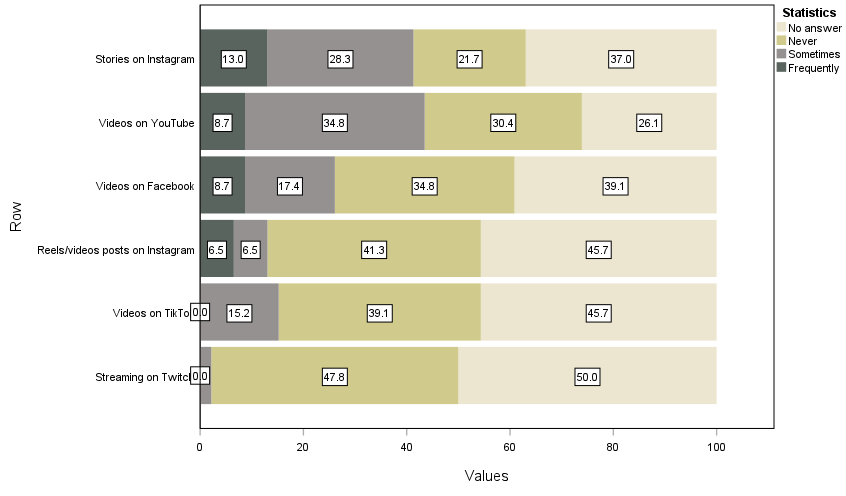
\includegraphics[width=\textwidth]{Fig-1.png}
\caption{Frequency of production of different types of videos.}
\label{fig-01}
\source{Own elaboration.}
\end{minipage}
\end{figure}

We also observe a pattern across all platforms, with the least common
response being to make videos frequently (from 13\% on Instagram to 0\%
on TikTok), indicating that a relatively low percentage of respondents
makes videos frequently, especially in comparison with the practice of
watching videos \cite{shafirova2023}. Moreover, we found a
correlation between the age of the students and the types of video
production. The correlation was found in the social media platforms of
TikTok, YouTube and Facebook, in which older students (older than 36)
tend to make videos for Facebook (due to cross tabulation with Pearson
chi-square test with 0.019 significance in case of YouTube and 0.004 in
case of Facebook). Meanwhile, younger students (from 18 to 23) tend to
make videos on TikTok (due to cross tabulation with Pearson chi-square
test with 0.008 significance). It is noteworthy that, on Instagram, we
did not find any correlation with age.

In general, in our data, age does not influence the frequency of making
videos, however, it points out that some social media platforms are more
frequently used by younger respondents and some by slightly older
respondents (similarly found in the dataset concerning the US population
from \textcite{ortizo-spina2019}). Moreover, the students post videos in
different languages, mostly in Portuguese and English (\Cref{tab-04}), while
other languages have a relatively smaller presence (max. 20\% with
Spanish on Facebook).

\begin{table}[htbp]
\centering
\begin{threeparttable}
\caption{Languages and platforms of video production: multiple choice response.}
\label{tab-04}
\begin{tabular}{*{11}{l}}
\toprule
Platforms & \multicolumn{2}{c}{YouTube} & \multicolumn{2}{c}{Facebook} &  \multicolumn{2}{c}{Instagram} & \multicolumn{2}{c}{TikTok} & \multicolumn{2}{c}{Twitch} \\
\midrule
Portuguese & 22 & 88\% & 13 & 86.7\% & 19 & 95\% & 5 & 71.4\% & 0 & 0\% \\
English    & 13 & 52\% & 6  & 40\%   & 9  & 45\% & 5 & 71.4\% & 1 & 50\% \\
Spanish    & 3  & 12\% & 3  & 20\%   & 1  & 5\%  & 0 & 0\%    & 0 & 0\% \\
Italian    & 2  & 8\%  & 2  & 13.3\% & 1  & 5\%  & 0 & 0\%    & 0 & 0\% \\
French     & 1  & 4\%  & 2  & 13.3\% & 0  & 0\%  & 0 & 0\%    & 0 & 0\% \\
Crioulo    & 0  & 0\%  & 0  & 0\%    & 1  & 5\%  & 0 & 0\%    & 0 & 0\% \\
Persian    & 0  & 0\%  & 1  & 6.7\%  & 0  & 0\%  & 0 & 0\%    & 0 & 0\% \\
Other      & 2  & 8\%  & 1  & 6.7\%  & 1  & 5\%  & 2 & 28.6\% & 1 & 50\% \\
\rule{0pt}{3ex}%
Total & 44 & 176\% & 28 & 186.7\% & 32 & 160\% & 12 & 171.4\% & 2 & 100\% \\
\bottomrule
\end{tabular}
\source{Own elaboration.}
\end{threeparttable}
\end{table}




In comparison, our previous study shows that video consumption on social
media and streaming platforms could be considered more diverse and
plurilingual. Even though English and Portuguese were still the most
popular languages, Spanish was used by roughly half of the participants
on streaming platforms such as Netflix and HBO. Additionally, such
languages as French, Italian, Korean or Japanese were also present, with
more than 10\% on various platforms \cite{shafirova2023}. There
could be various reasons for this difference in language variety in
video production and consumption. One possible explanation could be the
amount of resources available for watching videos in languages you do
not have a perfect command of, such as subtitles in different languages,
captions, scripts and more \cite{shafirova2023}.

Moreover, we asked the participants if they tended to use several
languages in one video. The participants responded with 26.1\% ``yes'',
with the main objective of reaching out to a vast audience (41.6\%), or
because of being multilingual (30\%).

\subsection{Why students make and post videos}

To understand students' intentions behind video production, we asked
about their objectives when making videos. According to \Cref{fig-02}, the
majority of the students make videos to ``have fun'' (63\%), which goes
along with previous research on video creation beyond the classroom
\cite{zhang2022}.

\begin{figure}[htbp]
\centering
\begin{minipage}{\textwidth}
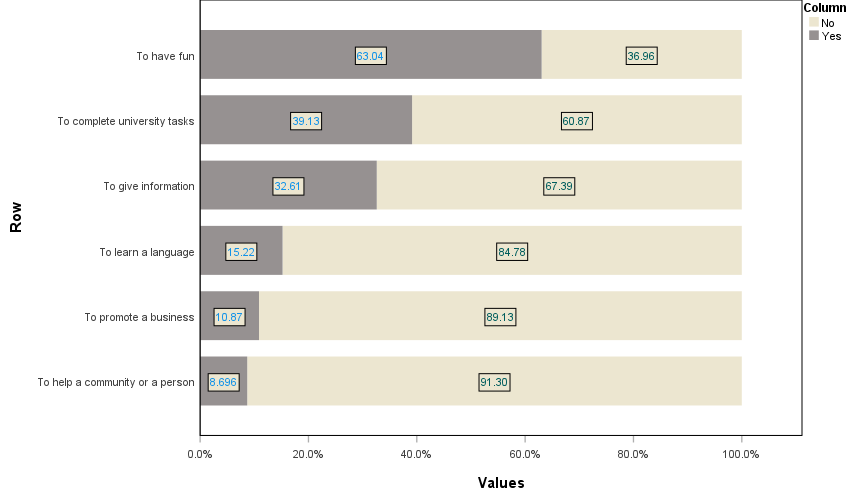
\includegraphics[width=\textwidth]{Fig-2.png}
\source{Own elaboration.}
\caption{Objectives to make videos.}
\label{fig-02}
\end{minipage}
\end{figure}

However, the second most popular answer is ``to complete university
tasks'' (39.1\%), which is a thought-provoking result indicating that
some of the university tasks require students to make videos (similar
results at the school level in \textcite{cassany2021}). It would be
valuable to explore the potential differences between the videos created
for leisure and those made as university tasks, even though these videos
would not necessarily be connected to language learning.

Moreover, the third answer was ``to give information'' (33\%), which
also seems like a serious and not entertaining goal, which can include
making videos or reposts of some news or events. This goes against the
assumption of some researchers that social media is always used only for
entertainment purposes \textcite{rosyida2019}. Also, the option ``to
learn a language'' was not popular (15.2\%), which is an expected result
as only 33\% of the participants are current language learners.

\subsection{What students do before and after producing videos}

Much like when watching videos online \cite{shafirova2023},
around half of the respondents were engaged in some communicative
actions before and after making a video. According to \Cref{tab-05} and \Cref{tab-06},
the communicative actions included searching (information or visuals),
reading (comments), writing (descriptions of the videos), watching
videos (to analyse similar videos), translating and interacting with
others (collaborating with others, responding to comments, making video
responses). The most frequent action before video production is
searching for information (\Cref{tab-05}), while the most frequent after
production is reading the comments or feedback on the videos (\Cref{tab-06}).
The options of writing descriptions or interacting with others were less
popular (roughly half of the responses).


\begin{table}[htbp]
\centering
\small
\begin{threeparttable}
\caption{Communicative actions made before video production.}
\label{tab-05}
\begin{tabular}{*{13}{l}}
\toprule
\multicolumn{1}{{>{\raggedright\arraybackslash}p{0.11\textwidth}}}{Actions} &
\multicolumn{2}{{>{\raggedright\arraybackslash}p{0.11\textwidth}}}{Search for information} &
\multicolumn{2}{{>{\raggedright\arraybackslash}p{0.11\textwidth}}}{Search for visual aid} &
\multicolumn{2}{{>{\raggedright\arraybackslash}p{0.11\textwidth}}}{Analyse similar videos} &
\multicolumn{2}{{>{\raggedright\arraybackslash}p{0.11\textwidth}}}{Write short descriptions} &
\multicolumn{2}{{>{\raggedright\arraybackslash}p{0.11\textwidth}}}{Collaborate with others} &
\multicolumn{2}{{>{\raggedright\arraybackslash}p{0.11\textwidth}}}{Make translations} \\
\midrule
Languages & N & \% & N & \% & N & \% & N & \% & N & \% & N & \% \\ 
Portuguese & 16 & 69.6\% & 11 & 47.8\% & 10 & 43.5\% & 11 & 47.8\% & 9  & 39.1\% & 7  & 30.4\% \\ 
English    & 18 & 78.3\% & 15 & 65.2\% & 11 & 47.8\% & 7  & 30.4\% & 7  & 30.4\% & 9  & 39.1\% \\ 
Spanish    & 3  & 13\%   & 2  & 8.7\%  & 3  & 13\%   & 1  & 4.3\%  & 2  & 8.7\%  & 1  & 4.3\%  \\ 
Italian    & 2  & 8.7\%  & 2  & 8.7\%  & 2  & 8.7\%  & 1  & 4.3\%  & 2  & 8.7\%  & 1  & 4.3\%  \\ 
French     & 2  & 8.7\%  & 2  & 8.7\%  & 2  & 8.7\%  & 0  & 0\%    & 2  & 8.7\%  & 1  & 4.3\%  \\ 
Chinese    & 1  & 4.3\%  & 1  & 4.3\%  & 0  & 0\%    & 1  & 4.3\%  & 0  & 0\%    & 0  & 0\%    \\ 
Persian    & 1  & 4.3\%  & 0  & 0\%    & 0  & 0\%    & 0  & 0\%    & 0  & 0\%    & 0  & 0\%    \\ 
Other      & 1  & 4.3\%  & 0  & 0\%    & 0  & 0\%    & 0  & 0\%    & 0  & 0\%    & 0  & 0\%    \\ 
\rule{0pt}{3ex}%
Total     & 44 & 191.2\% & 33 & 143.4\% & 28 & 121.7\% & 21 & 91.1\% & 22 & 95.6\% & 19 & 82.4\% \\ 
\bottomrule
\end{tabular}
\source{Own elaboration.}
\end{threeparttable}
\end{table}

Interestingly, if videos were mostly created in Portuguese and English,
the actions made before and after video production had more linguistic
variability, with the 7 languages present before video production, and
11 after production.

Furthermore, we made a comparison or cross-tabulation comparing the
participants\textquotesingle{} mother tongues with the actions taken
before video production (\Cref{tab-05}). The results showed that most
participants were using a foreign language before and after making a
video. In the case of activities made before video production, several
participants used such foreign languages as English, French and Italian.
Also, some participants used their mother tongues, including Portuguese,
Spanish, Chinese and Persian. Similar data emerged when comparing the
responses concerning the actions taken after posting the videos in
relation to the participants' mother tongues (\Cref{tab-06}).


\begin{table}[htbp]
\centering
\begin{threeparttable}
\caption{Communicative actions made after video production.}
\label{tab-06}
\begin{tabular}{*{7}{l}}
\toprule
Actions &
\multicolumn{2}{{{>{\raggedright\arraybackslash}p{0.25\textwidth}}}}{Read comments, chat, reactions} &
\multicolumn{2}{{>{\raggedright\arraybackslash}p{0.14285714285\textwidth}}}{Respond to the comments} &
\multicolumn{2}{{>{\raggedright\arraybackslash}p{0.14285714285\textwidth}}}{Make video responses to comments} \\
\midrule
Portuguese & 19 & 79.2\% & 8 & 33.3\% & 3 & 12.5\% \\ 
English    & 17 & 70.8\% & 9 & 37.5\% & 3 & 12.5\% \\ 
Spanish    & 7  & 29.2\% & 3 & 12.5\% & 1 & 4.2\%  \\ 
Italian    & 5  & 20.8\% & 3 & 12.5\% & 1 & 4.2\%  \\ 
French     & 5  & 20.8\% & 2 & 8.3\%  & 2 & 8.3\%  \\ 
Chinese    & 2  & 8.3\%  & 1 & 4.2\%  & 1 & 4.2\%  \\ 
Persian    & 2  & 8.3\%  & 1 & 4.2\%  & 2 & 8.3\%  \\ 
Russian    & 2  & 8.3\%  & 1 & 4.2\%  & 1 & 4.2\%  \\ 
Korean     & 1  & 4.2\%  & 1 & 4.2\%  & 1 & 4.2\%  \\ 
Crioulo    & 1  & 4.2\%  & 1 & 4.2\%  & 1 & 4.2\%  \\ 
Japanese   & 1  & 4.2\%  & 1 & 4.2\%  & 1 & 4.2\%  \\ 
Other      & 1  & 4.2\%  & 1 & 4.2\%  & 2 & 8.3\%  \\ 
Total      & 63 & 262.5\% & 32 & 133.5\% & 19 & 79.3\% \\ 
\bottomrule
\end{tabular}
\source{Own elaboration.}
\end{threeparttable}
\end{table}

For instance, in \Cref{tab-06}, most participants used English as a foreign
language when reading and responding to comments. Other foreign
languages included Spanish (only one respondent used it as a mother
tongue), French, Italian and Korean. These data indicate that students
engaged in communicative activities in foreign languages both before and
after making a video. This characterizes video production as interactive
and increases language input through various modes, including written,
oral, interactive, and information-seeking activities.

\subsection{The students' perceptions of language learning with video production and consumption}

The questionnaire included two questions about students' perceptions of
language learning while watching or producing videos. The questions went
as follows: ``To what extent do you agree with the statement:
Watching/producing videos in (an)other language(s) helped me in learning
this(ese) language(s)''.

In \Cref{fig-03}, we compare the answers to these questions divided into two
graphics (based on N-46), one focused on video viewing (blue) and the
other on video production (red). The line on video viewing is much more
accentuated in comparison with video production which has an almost
normal distribution.

\begin{figure}[htbp]
\centering
\begin{minipage}{\textwidth}
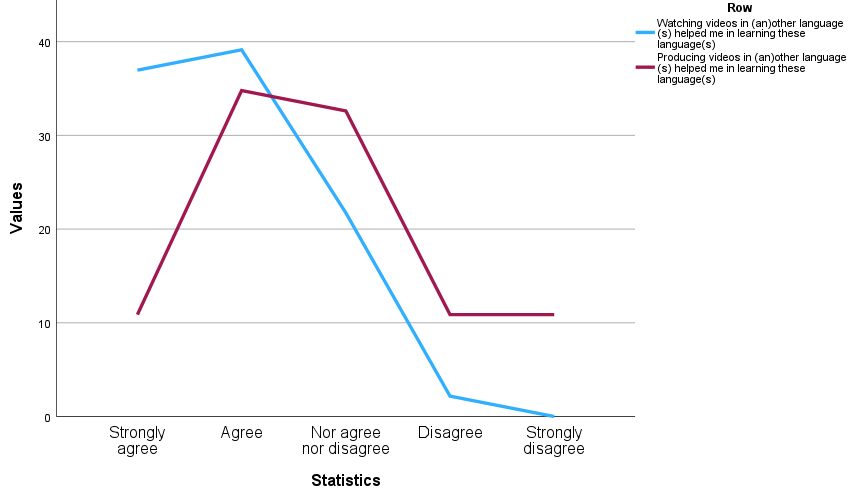
\includegraphics[width=\textwidth]{Fig-3.png}
\caption{Students' perceptions of language learning with the help
	of video watching/producing.}
\label{fig-03}
\source{Own elaboration.}
\end{minipage}
\end{figure}

It indicates that in the case of video watching, the students mostly
``strongly agree'' and ``agree'' (around 75\%) with the proposed
statement. However, in the case of video producing, most respondents
``agree'' or ``neither agree nor disagree'' (around 70\%), with some
respondents ``disagreeing'' and ``strongly disagreeing'' (around 22\%).
This comparison shows a division in opinions on the benefits of video
production, with more uncertainty in the results for video production
compared with video watching.

These results could be connected to the frequency of video production
compared to video viewing and the fact that students could be engaged in
very different forms of video production, from Instagram stories to
lengthy videos on YouTube. It can also be connected to our particular
dataset which includes students from non-language studies. In general,
we consider this discrepancy in data on video viewing and production an
interesting phenomenon for further investigation.

Additionally, we ran a cross-tabulation test with a Pearson Chi-Square
test to examine if there is a correlation between these students'
perceptions of video production (\Cref{fig-03}) and the fact that they are
current language learners (\Cref{tab-03}). The p-value (or significance) for
the Chi-Square test was 0.6, indicating no significant correlation
between these two variables. However, due to the small sample size,
seven cells had an expected count of less than 5, which may make the
results unreliable. To address this, we combined the cells ``agree'' and
``strongly agree,'' as well as ``disagree'' and ``strongly disagree,''
transforming the 5-level Likert scale into a 3-level scale. In this
adjusted analysis, only two cells had an expected count of less than 5,
making the results more reliable. Similar to the previous test, the
p-value was 0.3, indicating no significant correlation between these
categories. In addition, we ran the Fisher Exact test which is better
suited for smaller samples, nevertheless, it also did not indicate any
correlation ($p=0.7$ in the first case and $p=9.4$ in the second case).

These results indicate that there is no significant correlation between
these two categories. We also examined the categories of current
language learners and students\textquotesingle{} perceptions of video
watching, and similarly found no correlation (Chi-Square test, $p=0.5$;
Fisher Exact test, $p=0.7$). However, it would be beneficial to test this
hypothesis with a larger dataset to confirm these findings.

Moreover, we examined the relationship between the category of students'
perceptions of video production benefits and the departments where the
students study. We combined our categories into 1) Language Department,
2) Education and Psychology, and 3) Other to see if there are some
correlations between our specific dataset and the question. The
Chi-Square test showed no significant correlation $(p= 0.066)$, however,
the Fisher Exact test showed some significance $(p = 0.05)$. In this case,
as our dataset is small and 50\% of the results have an expected count
of less than 5, the Fisher Exact Test seems to be more reliable \cite{jung2014}.
\Cref{fig-04} also shows a strong indication of dependence between
these categories.

\begin{figure}[htbp]
\centering
\begin{minipage}{\textwidth}
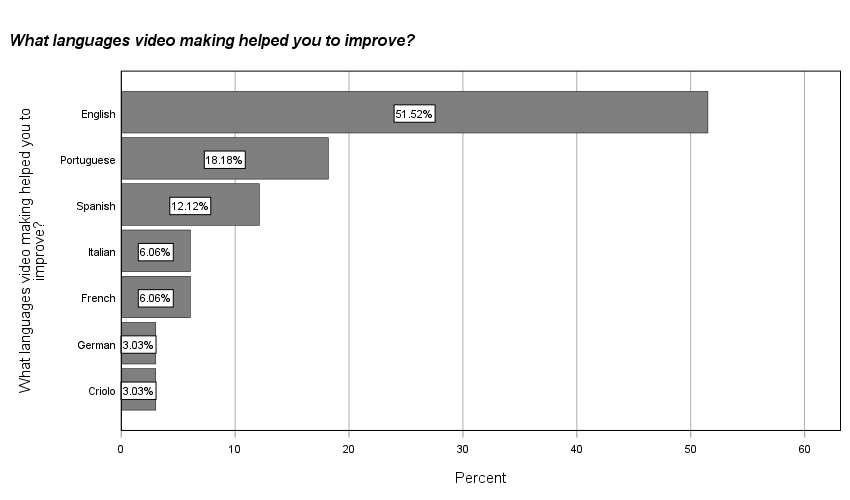
\includegraphics[width=\textwidth]{Fig-4.png}
\caption{Perceptions of the students on video production:
	department distribution.}
\label{fig-04}
\source{Own elaboration.}
\end{minipage}
\end{figure}

According to \Cref{fig-04}, we can see that in the Languages and Cultures
department, most students agree that video production helps in learning
a language (adjusted residual 1.6), while in Other Departments fewer
people agree with this statement (adjusted residual -2.5). In the
Department of Education and Psychology, fewer students disagreed that
video production could help language learning (adjusted residual -1.8).
The distribution observed here indicates more positive perceptions of
video production in the Department of Languages and Cultures. This
suggests that teaching methodologies in the Languages and Cultures and
the Education and Psychology departments may be influencing
students\textquotesingle{} perceptions. Additionally, when we tested the
correlation between a departmental distribution and students'
perceptions of video watching, we found no significant correlation using
either the Chi-Square test $(p=0.3)$ or the Fisher Exact test $(p=0.3)$.
Examining this question across different departments would be
beneficial, as our current dataset is too small to draw definitive
conclusions.

Moreover, 46\% of students chose the categories ``strongly agree'' and
``agree'' with the benefits of video production for language learning.
They also answered the next question regarding the languages that
video-making helped them learn (\Cref{tab-05}).

\begin{figure}[htbp]
\centering
\begin{minipage}{\textwidth}
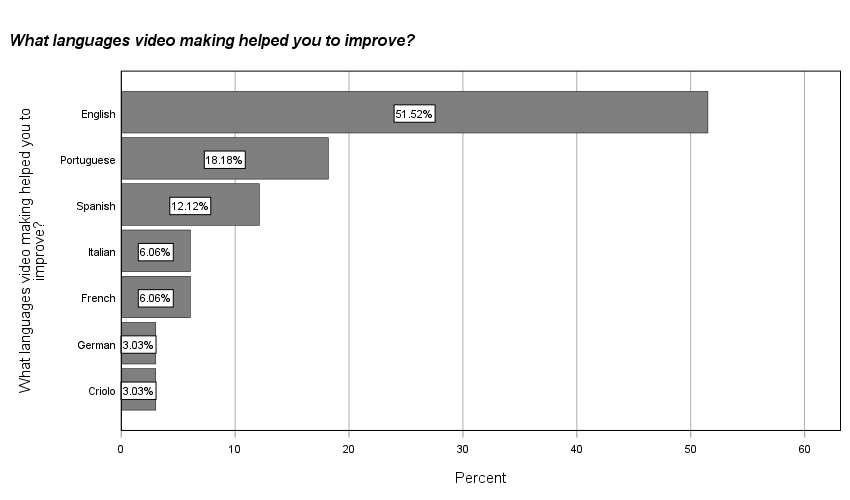
\includegraphics[width=\textwidth]{Fig-5.png}
\caption{Languages improved by making videos}
\label{fig-05}
\source{Own elaboration.}
\end{minipage}
\end{figure}

According to \Cref{fig-05}, the respondents chose a considerable variety of
languages, taking into account that only 21 people (from 46) responded
to that question and chose seven languages. English was the most popular
response, followed by Portuguese and Spanish. Notably, we can also see
\emph{Crioulo} derived from the Portuguese language (variation from Cabo
Verde) in the responses, which was completely absent from video viewing
responses \cite{shafirova2023}.

The students also responded to an open question concerning language
learning and video viewing/production: ``How have you improved your
language and cultural skills by watching/producing videos in different
languages?'' In the case of video viewing, we received 52 responses or
around 25\% of 212 respondents. According to our codebook (\Cref{annex-a}), 23
responses included the learning of vocabulary, oral comprehension had 9
responses, and pronunciation had 7. Students also noticed learning the
cultural aspects (7) of countries where languages are used and
underlined the importance of learning the language in the context of its
use (5). Overall, the detailed responses indicate that students view
this knowledge as important to share.

In the case of video production, we received 8 responses out of 46, in
other words, 17\% of the students responded, including such categories
as vocabulary (4), speaking (2) and cultural aspects (1). The answers
were less detailed than those in the viewing section, with a lower
overall response rate. Additionally, most responses came from the
Departments of Languages and Cultures and Education and Psychology. Some
responses highlighted that not only video production was beneficial for
language learning but also the work completed beforehand or afterwards
(\Cref{annex-a}). For instance, one respondent noticed: ``The research required
to produce most of my content has allowed me to widen my vision of the
English language and culture''.

We observe that students frequently highlighted vocabulary as the
primary area of improvement in both video viewing and production. This
suggests that, from the respondents\textquotesingle{} perspective,
vocabulary could be the most beneficial aspect of both practices.
%
\section{Funding}\label{sec-funding}
This work is funded by national funds through FCT – Fundação para a Ciência e a Tecnologia, I.P., under the Scientific Employment Stimulus - Individual Call – [2022.06443.CEECIND] and the CIDTFF Research Centre (projects UIDB/00194/2020 and UIDP/00194/2020). It was also partly supported by OralGrab. Grabar vídeos y audios para ensenyar y aprender (PID2022-141511NB-100, Ministry of Science and Innovation), Gr@el - Grup de recerca sobre aprenentatge i ensenyament de llengües (SGR471, AGAUR), and by DEFINERS: Digital language learning of language teachers (TED2021-129984A-I00, Ministry of Science and Innovation, Spain).


\printbibliography
\label{sec-bib}
%conceptualization,datacuration,formalanalysis,funding,investigation,methodology,projadm,resources,software,supervision,validation,visualization,writing,review
\begin{contributors}[sec-contributors]
\authorcontribution{Leonardo Araújo}[conceptualization,datacuration,formalanalysis,investigation,methodology,software,validation,visualization,writing,review]
\authorcontribution{Daniervelin Pereira}[methodology,projadm,resources,validation,writing,review]
\end{contributors}

\newpage
\section{Anexo 1}\label{appdx1}

% Save the original values of LTleft and LTright
\newlength{\originalLTleft}
\setlength{\originalLTleft}{\LTleft}
\newlength{\originalLTright}
\setlength{\originalLTright}{\LTright}
\setlength\LTleft{-2cm}
\setlength\LTright{-2cm}
\begin{footnotesize}
\begin{longtable}{l >{\raggedright}p{2cm} *{8}{l}}
\caption{Resultados de los 28 ítems elaborados por ChatGPT 4.0}
\label{tab-12}\\
\toprule
No. & Tema & \multicolumn{1}{>{\raggedright}p{1.2cm}}{Demanda cognitiva} & \multicolumn{1}{>{\raggedright}p{1.2cm}}{Dificultad} & \multicolumn{1}{>{\raggedright}p{1.2cm}}{Infit MNSQ} & \multicolumn{1}{>{\raggedright}p{1.2cm}}{Infit ZSTD} & \multicolumn{1}{>{\raggedright}p{1.2cm}}{Outfit MNSQ} & \multicolumn{1}{>{\raggedright}p{1.2cm}}{Outfit ZSTD} & \multicolumn{1}{>{\raggedright}p{1.2cm}}{Corr. Punto-biserial} & \multicolumn{1}{>{\raggedright}p{1.2cm}}{Discriminación} \\
\midrule
	1 & Uso de palabras en oraciones & Evaluación & 0.39 & 0.93 & -0.8 & 0.85 & -1.1 & 0.35 & 1.16 \\
	2 & Uso de palabras en oraciones & Evaluación & 0.65 & 1.13 & 0.9 & 1.27
	& 1.4 & 0.01 & 0.81 \\
	3 & Uso de palabras en oraciones & Evaluación & 0.68 & 1.07 & 0.5 & 1.26
	& 1.1 & 0.04 & 0.9 \\
	4 & Uso de palabras en oraciones & Evaluación & 0.56 & 0.96 & -0.6 &
	0.96 & -0.4 & 0.32 & 1.12 \\
	5 & Economía del lenguaje & Evaluación & 0.56 & 1.05 & 0.7 & 1.07 & 0.8
	& 0.19 & 0.82 \\
	6 & Economía del lenguaje & Evaluación & 0.58 & 1.07 & 0.9 & 1.1 & 0.9 &
	0.14 & 0.79 \\
	7 & Economía del lenguaje & Evaluación & 0.55 & 1.12 & 1.8 & 1.17 & 1.9
	& 0.05 & 0.52 \\
	8 & Economía del lenguaje & Evaluación & 0.53 & 0.95 & -0.9 & 0.93 & -1
	& 0.34 & 1.23 \\
	9 & Uso efectivo de la semántica & Evaluación & 0.6 & 1.08 & 1 & 1.1 &
	0.7 & 0.13 & 0.82 \\
	10 & Uso efectivo de la semántica & Evaluación & 0.28 & 0.96 & -0.2 &
	0.82 & -0.6 & 0.25 & 1.05 \\
	11 & Uso efectivo de la semántica & Evaluación & 0.77 & 1.07 & 0.3 & 1.3
	& 0.8 & 0 & 0.93 \\
	12 & Uso efectivo de la semántica & Evaluación & 0.81 & 1.05 & 0.2 &
	1.87 & 1.6 & -0.06 & 0.92 \\
	13 & Uso efectivo de la semántica & Evaluación & 0.6 & 1 & 0 & 1.04 &
	0.3 & 0.23 & 0.98 \\
	14 & Concordancia entre sujeto y verbo & Aplicación & 0.68 & 1.05 & 0.3
	& 1.19 & 0.8 & 0.1 & 0.93 \\
	15 & Concordancia entre sujeto y verbo & Aplicación & 0.51 & 1.05 & 0.9
	& 1.06 & 0.9 & 0.18 & 0.75 \\
	16 & Concordancia entre sujeto y verbo & Aplicación & 0.51 & 0.98 & -0.4
	& 0.96 & -0.5 & 0.28 & 1.13 \\
	17 & Concordancia entre sujeto y verbo & Aplicación & 0.49 & 0.89 & -2.3
	& 0.87 & -2 & 0.42 & 1.64 \\
	18 & Concordancia entre sujeto y verbo & Aplicación & 0.48 & 0.87 & -2.4
	& 0.84 & -2.1 & 0.45 & 1.63 \\
	19 & Convenciones de puntuación: coma & Aplicación & 0.62 & 1.01 & 0.1 &
	1.1 & 0.7 & 0.2 & 0.95 \\
	20 & Convenciones de puntuación: coma & Aplicación & 0.42 & 0.94 & -0.8
	& 0.9 & -1 & 0.33 & 1.17 \\
	21 & Convenciones de puntuación: coma & Aplicación & 0.51 & 0.94 & -1.1
	& 0.93 & -1 & 0.34 & 1.31 \\
	22 & Convenciones de puntuación: coma & Aplicación & 0.57 & 1.07 & 0.9 &
	1.11 & 1 & 0.16 & 0.79 \\
	23 & Convenciones de puntuación: coma & Aplicación & 0.58 & 1.03 & 0.4 &
	1.08 & 0.7 & 0.19 & 0.88 \\
	24 & Convenciones de puntuación: interrogación & Aplicación & 0.43 &
	0.92 & -1.1 & 0.87 & -1.2 & 0.37 & 1.26 \\
	25 & Convenciones de puntuación: interrogación & Aplicación & 0.51 &
	1.01 & 0.2 & 1 & 0.1 & 0.24 & 0.96 \\
	26 & Convenciones de puntuación: interrogación & Aplicación & 0.44 &
	0.88 & -1.9 & 0.85 & -1.8 & 0.42 & 1.44 \\
	27 & Convenciones de puntuación: interrogación & Aplicación & 0.42 &
	0.88 & -1.6 & 0.84 & -1.5 & 0.42 & 1.32 \\
	28 & Convenciones de puntuación: interrogación & Aplicación & 0.63 &
	1.13 & 1.2 & 1.26 & 1.4 & 0.03 & 0.77 \\	
\multicolumn{3}{r}{Promedio general} & 0.55 & 1.00 & -0.14 & 1.06 & 0.03 & 0.22 & 1.04 \\
\bottomrule
\source{Elaboración propia.}
\end{longtable}
\end{footnotesize}
% Revert to the original values
\setlength\LTleft{\originalLTleft}
\setlength\LTright{\originalLTright}



\section{Anexo 2}
\setlength\LTleft{-0.125cm}
\setlength\LTright{-0.125cm}
\begin{footnotesize}
\begin{longtable}{llll}
\caption{Datos de las evaluaciones por creador y Juez}
\label{tab-13}
\\
\toprule
Creador & Evaluación Juez A & Evaluación Juez B & Evaluación ChatGPT \\
\midrule
	ChatGPT & 1 & 0 & 0 \\
	ChatGPT & 2 & 2 & 2 \\
	ChatGPT & 1 & 0 & 0 \\
	ChatGPT & 1 & 0 & 0 \\
	ChatGPT & 1 & 0 & 0 \\
	ChatGPT & 1 & 0 & 0 \\
	ChatGPT & 0 & 0 & 0 \\
	ChatGPT & 1 & 0 & 0 \\
	ChatGPT & 2 & 0 & 0 \\
	ChatGPT & 0 & 0 & 0 \\
	ChatGPT & 0 & 0 & 0 \\
	ChatGPT & 0 & 0 & 0 \\
	ChatGPT & 0 & 0 & 0 \\
	ChatGPT & 0 & 0 & 0 \\
	ChatGPT & 0 & 0 & 0 \\
	ChatGPT & 2 & 0 & 0 \\
	ChatGPT & 0 & 0 & 0 \\
	ChatGPT & 2 & 0 & 0 \\
	ChatGPT & 0 & 0 & 0 \\
	ChatGPT & 2 & 0 & 0 \\
	ChatGPT & 3 & 0 & 1 \\
	ChatGPT & 0 & 0 & 0 \\
	ChatGPT & 0 & 0 & 0 \\
	ChatGPT & 2 & 0 & 0 \\
	ChatGPT & 2 & 0 & 0 \\
	ChatGPT & 2 & 0 & 0 \\
	ChatGPT & 2 & 0 & 0 \\
	ChatGPT & 2 & 0 & 0 \\
	Humano & 1 & 0 & 0 \\
	Humano & 0 & 0 & 0 \\
	Humano & 1 & 0 & 0 \\
	Humano & 1 & 0 & 0 \\
	Humano & 0 & 0 & 0 \\
	Humano & 1 & 0 & 0 \\
	Humano & 0 & 0 & 0 \\
	Humano & 2 & 0 & 0 \\
	Humano & 0 & 0 & 0 \\
	Humano & 0 & 0 & 0 \\
	Humano & 0 & 0 & 0 \\
	Humano & 2 & 0 & 0 \\
	Humano & 0 & 0 & 0 \\
	Humano & 0 & 0 & 0 \\
	Humano & 1 & 2 & 2 \\
	Humano & 0 & 0 & 0 \\
	Humano & 0 & 0 & 0 \\
	Humano & 0 & 0 & 0 \\
	Humano & 0 & 0 & 0 \\
	Humano & 2 & 2 & 0 \\
	Humano & 2 & 2 & 0 \\
	Humano & 0 & 2 & 0 \\
	Humano & 0 & 0 & 0 \\
	Humano & 2 & 0 & 0 \\
	Humano & 2 & 0 & 0 \\
	Humano & 0 & 0 & 0 \\
	Humano & 3 & 0 & 0 \\
	Humano & 1 & 0 & 1 \\
	Humano & 2 & 0 & 0 \\
	Humano & 0 & 0 & 0 \\
	Humano & 0 & 0 & 0 \\
	Humano & 2 & 0 & 0 \\
	Humano & 1 & 0 & 0 \\
	Humano & 1 & 0 & 1 \\
	Humano & 0 & 0 & 0 \\
	Humano & 0 & 0 & 0 \\
	Humano & 2 & 0 & 0 \\
	Humano & 2 & 0 & 0 \\
	Humano & 2 & 0 & 0 \\
	Humano & 2 & 0 & 0 \\
	Humano & 2 & 0 & 0 \\
	Humano & 2 & 0 & 0 \\
	Humano & 2 & 0 & 0 \\
	Humano & 2 & 0 & 0 \\
	Humano & 0 & 0 & 0 \\
	Humano & 2 & 2 & 2 \\
	Humano & 2 & 2 & 0 \\
	Humano & 0 & 0 & 0 \\
	Humano & 2 & 0 & 0 \\
	Humano & 2 & 0 & 0 \\
	Humano & 2 & 0 & 0 \\
	Humano & 0 & 0 & 0 \\
	Humano & 2 & 0 & 0 \\
	Humano & 2 & 0 & 0 \\
	Humano & 2 & 0 & 0 \\
	Humano & 2 & 0 & 0 \\
\bottomrule 
\source{Elaboración propia.} \\
\addlinespace
\multicolumn{4}{l}{\footnotesize
	Sin cambio = 0; Con cambios menores = 1; Con cambios mayores = 2;
	Rechazado = 3.}\\
\end{longtable}
\end{footnotesize}


\end{document}
